\section*{Simulated Total Energy vs. Time (varying e)}

% sim-001 total energy
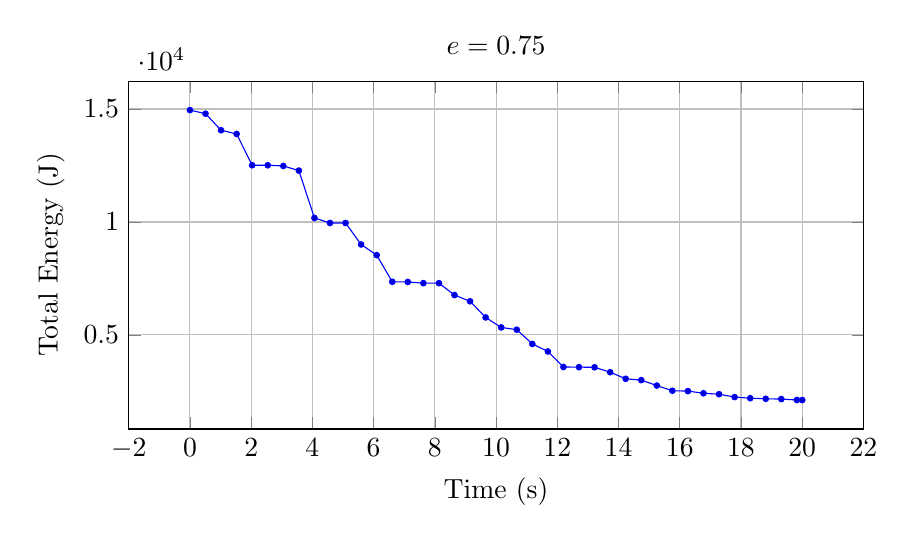
\begin{tikzpicture}
\begin{axis}[
    width=0.9\textwidth,
    height=6cm,
    xlabel={Time (s)},
    ylabel={Total Energy (J)},
    title={$e = 0.75$},
    grid=both,
    tick label style={/pgf/number format/fixed},
]
\addplot+[mark=*, mark size=1pt] coordinates {
(0.0,14952.35)
(0.5083333313000006,14793.449377865778)
(1.0166666625999987,14060.99750925699)
(1.5249999938999967,13896.477440682682)
(2.0333333251999948,12510.882701954857)
(2.541666656499993,12510.88270195486)
(3.049999987799991,12479.417453684833)
(3.558333319099989,12273.363378570186)
(4.06666665039999,10177.437401698673)
(4.5749999817000155,9953.755916310372)
(5.083333313000041,9953.755916310378)
(5.591666644300066,9002.041334518524)
(6.099999975600091,8530.583665838883)
(6.608333306900116,7350.988837906317)
(7.116666638200141,7342.441980877146)
(7.624999969500166,7290.264841132356)
(8.133333300800178,7290.264841132361)
(8.641666632100149,6763.498647989738)
(9.14999996340012,6487.124076635238)
(9.65833329470009,5772.572317610013)
(10.166666626000062,5329.722018976285)
(10.674999957300033,5230.0151650428525)
(11.183333288600004,4599.122403695114)
(11.691666619899975,4264.852754860962)
(12.199999951199946,3578.1682360247087)
(12.708333282499916,3570.672635253077)
(13.216666613799887,3564.085241381409)
(13.724999945099858,3347.1138177804833)
(14.23333327639983,3054.998878267983)
(14.7416666076998,2997.0310074787008)
(15.249999938999771,2756.1710588494307)
(15.758333270299742,2526.3793017135954)
(16.26666660159977,2510.3000125844205)
(16.77499993289985,2414.674124740351)
(17.28333326419993,2373.3887490235866)
(17.791666595500008,2245.9090397318696)
(18.299999926800087,2195.9169572877395)
(18.808333258100166,2169.7127961186698)
(19.316666589400246,2157.634562192314)
(19.824999920700325,2117.2402358938666)
(19.999999920000352,2114.986428980833)
};
\end{axis}
\end{tikzpicture}


% sim-002 total energy
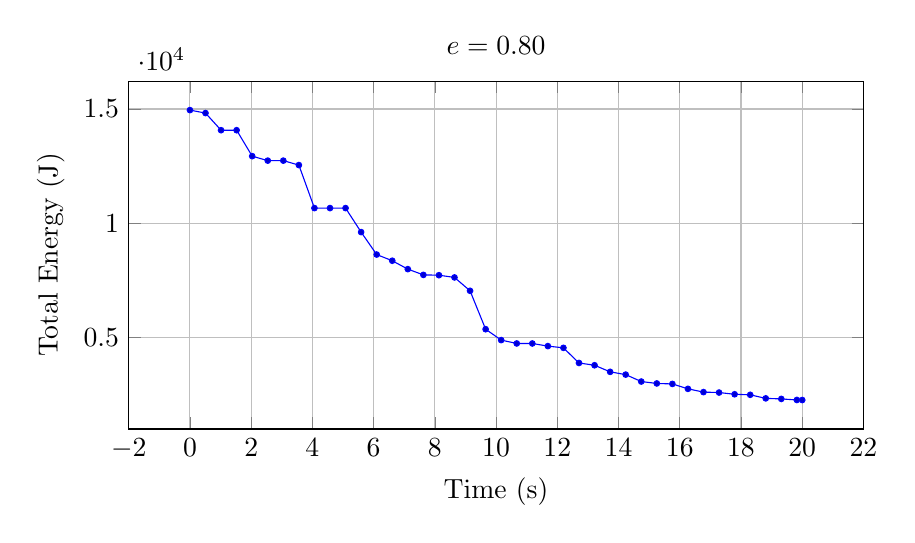
\begin{tikzpicture}
\begin{axis}[
    width=0.9\textwidth,
    height=6cm,
    xlabel={Time (s)},
    ylabel={Total Energy (J)},
    title={$e = 0.80$},
    grid=both,
    tick label style={/pgf/number format/fixed},
]
\addplot+[mark=*, mark size=1pt] coordinates {
(0.0,14952.35)
(0.5083333313000006,14821.69007714793)
(1.0166666625999987,14071.647349413635)
(1.5249999938999967,14071.647349413639)
(2.0333333251999948,12934.244846683321)
(2.541666656499993,12738.379122106688)
(3.049999987799991,12738.379122106693)
(3.558333319099989,12543.228484878187)
(4.06666665039999,10658.38604491867)
(4.5749999817000155,10658.386044918667)
(5.083333313000041,10658.386044918669)
(5.591666644300066,9605.809429482122)
(6.099999975600091,8623.339413409078)
(6.608333306900116,8351.50728562189)
(7.116666638200141,7984.009455230087)
(7.624999969500166,7731.31373067596)
(8.133333300800178,7718.229943083752)
(8.641666632100149,7619.9053856341325)
(9.14999996340012,7033.329538183809)
(9.65833329470009,5352.004190407549)
(10.166666626000062,4873.502175461628)
(10.674999957300033,4726.972847669426)
(11.183333288600004,4725.859533409453)
(11.691666619899975,4610.8075076882615)
(12.199999951199946,4534.565748084708)
(12.708333282499916,3871.624178330014)
(13.216666613799887,3771.282518514108)
(13.724999945099858,3482.468425705953)
(14.23333327639983,3361.8662908606675)
(14.7416666076998,3057.949471982987)
(15.249999938999771,2973.928964419454)
(15.758333270299742,2953.5395957848323)
(16.26666660159977,2738.0024987456713)
(16.77499993289985,2594.9732927669647)
(17.28333326419993,2576.14073308934)
(17.791666595500008,2499.6341183852155)
(18.299999926800087,2476.2558583775617)
(18.808333258100166,2321.2826192069074)
(19.316666589400246,2296.6136211563776)
(19.824999920700325,2251.026132346474)
(19.999999920000352,2247.8934615111625)
};
\end{axis}
\end{tikzpicture}


% sim-003 total energy
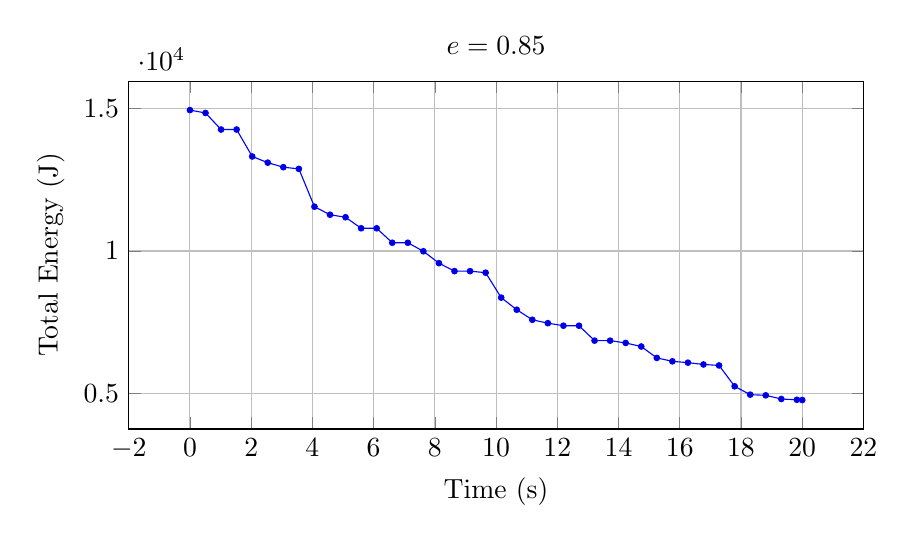
\begin{tikzpicture}
\begin{axis}[
    width=0.9\textwidth,
    height=6cm,
    xlabel={Time (s)},
    ylabel={Total Energy (J)},
    title={$e = 0.85$},
    grid=both,
    tick label style={/pgf/number format/fixed},
]
\addplot+[mark=*, mark size=1pt] coordinates {
(0.0,14952.35)
(0.5083333313000006,14851.752757028931)
(1.0166666625999987,14269.774127311952)
(1.5249999938999967,14269.774127311957)
(2.0333333251999948,13324.09087755664)
(2.541666656499993,13105.777090489755)
(3.049999987799991,12945.833592323303)
(3.558333319099989,12887.07269580071)
(4.06666665039999,11558.32581884131)
(4.5749999817000155,11276.214354634007)
(5.083333313000041,11187.020904263554)
(5.591666644300066,10799.783953241065)
(6.099999975600091,10799.783953241067)
(6.608333306900116,10291.540733043772)
(7.116666638200141,10291.540733043774)
(7.624999969500166,9992.097843827984)
(8.133333300800178,9574.687556423729)
(8.641666632100149,9293.931012948942)
(9.14999996340012,9293.931012948946)
(9.65833329470009,9240.14829450998)
(10.166666626000062,8363.266171947203)
(10.674999957300033,7938.199364991653)
(11.183333288600004,7584.849294897862)
(11.691666619899975,7465.314625225458)
(12.199999951199946,7376.622078878891)
(12.708333282499916,7376.622078878893)
(13.216666613799887,6852.383960030509)
(13.724999945099858,6852.383960030509)
(14.23333327639983,6770.419131491028)
(14.7416666076998,6645.620708364326)
(15.249999938999771,6245.550147907972)
(15.758333270299742,6124.800404880835)
(16.26666660159977,6078.160465102783)
(16.77499993289985,6014.876037743097)
(17.28333326419993,5980.574755501706)
(17.791666595500008,5247.79596518493)
(18.299999926800087,4954.183959951206)
(18.808333258100166,4929.9300151061025)
(19.316666589400246,4801.025100072453)
(19.824999920700325,4774.244710367897)
(19.999999920000352,4765.0503661848115)
};
\end{axis}
\end{tikzpicture}


% sim-004 total energy
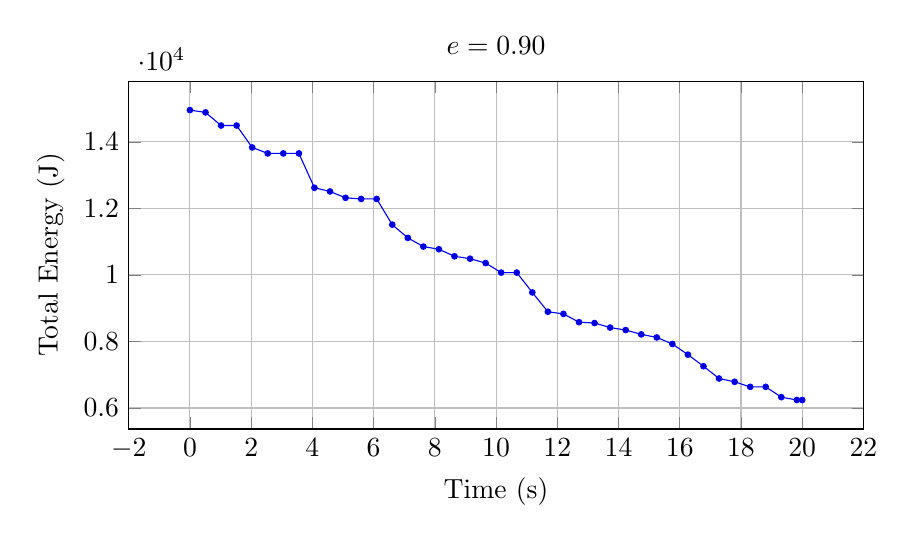
\begin{tikzpicture}
\begin{axis}[
    width=0.9\textwidth,
    height=6cm,
    xlabel={Time (s)},
    ylabel={Total Energy (J)},
    title={$e = 0.90$},
    grid=both,
    tick label style={/pgf/number format/fixed},
]
\addplot+[mark=*, mark size=1pt] coordinates {
(0.0,14952.35)
(0.5083333313000006,14883.637417508777)
(1.0166666625999987,14488.391569414702)
(1.5249999938999967,14488.391569414707)
(2.0333333251999948,13829.669651831377)
(2.541666656499993,13650.30903544757)
(3.049999987799991,13650.309035447572)
(3.558333319099989,13650.309035447579)
(4.06666665039999,12617.675594326334)
(4.5749999817000155,12506.993280713672)
(5.083333313000041,12315.57246875409)
(5.591666644300066,12282.231860066082)
(6.099999975600091,12282.231860066086)
(6.608333306900116,11509.505184735082)
(7.116666638200141,11111.630001406054)
(7.624999969500166,10850.701433943392)
(8.133333300800178,10770.007503233082)
(8.641666632100149,10559.056507093683)
(9.14999996340012,10485.739489145748)
(9.65833329470009,10355.050610290382)
(10.166666626000062,10068.334431774927)
(10.674999957300033,10068.334431774938)
(11.183333288600004,9472.32074139948)
(11.691666619899975,8891.811344193096)
(12.199999951199946,8826.64482766262)
(12.708333282499916,8578.738336519204)
(13.216666613799887,8552.015175675047)
(13.724999945099858,8416.75900832302)
(14.23333327639983,8341.365578060699)
(14.7416666076998,8212.060450930816)
(15.249999938999771,8119.604128347984)
(15.758333270299742,7922.127945247138)
(16.26666660159977,7601.79178488001)
(16.77499993289985,7253.939646604871)
(17.28333326419993,6885.187327559558)
(17.791666595500008,6785.7942797142405)
(18.299999926800087,6634.20852235607)
(18.808333258100166,6634.208522356072)
(19.316666589400246,6324.424683354282)
(19.824999920700325,6238.8247721669595)
(19.999999920000352,6238.8247721669595)
};
\end{axis}
\end{tikzpicture}


% sim-005 total energy
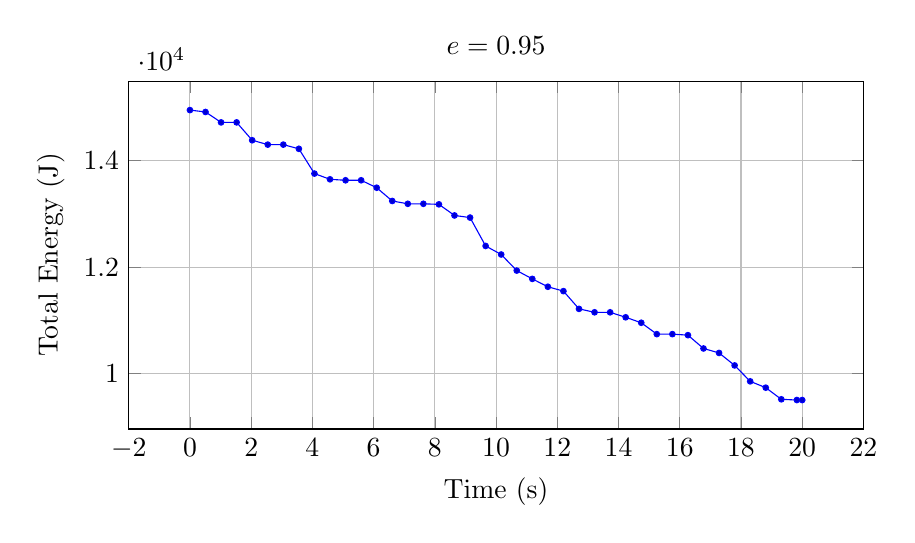
\begin{tikzpicture}
\begin{axis}[
    width=0.9\textwidth,
    height=6cm,
    xlabel={Time (s)},
    ylabel={Total Energy (J)},
    title={$e = 0.95$},
    grid=both,
    tick label style={/pgf/number format/fixed},
]
\addplot+[mark=*, mark size=1pt] coordinates {
(0.0,14952.35)
(0.5083333313000006,14917.344058587474)
(1.0166666625999987,14721.297834707682)
(1.5249999938999967,14721.297834707688)
(2.0333333251999948,14385.709382792906)
(2.541666656499993,14303.327247480476)
(3.049999987799991,14303.327247480478)
(3.558333319099989,14224.456354241931)
(4.06666665039999,13758.78596468365)
(4.5749999817000155,13651.011602345641)
(5.083333313000041,13632.873725656009)
(5.591666644300066,13632.873725656007)
(6.099999975600091,13492.80977177181)
(6.608333306900116,13243.516785691252)
(7.116666638200141,13190.430226717777)
(7.624999969500166,13190.430226717774)
(8.133333300800178,13179.932187211783)
(8.641666632100149,12971.439398971932)
(9.14999996340012,12931.391408916594)
(9.65833329470009,12398.047163211495)
(10.166666626000062,12237.073166969152)
(10.674999957300033,11935.032861552918)
(11.183333288600004,11778.632063766778)
(11.691666619899975,11630.79688501585)
(12.199999951199946,11548.41113239637)
(12.708333282499916,11214.734162165641)
(13.216666613799887,11150.200307127694)
(13.724999945099858,11150.200307127694)
(14.23333327639983,11056.409146557951)
(14.7416666076998,10953.76940471673)
(15.249999938999771,10739.834609102109)
(15.758333270299742,10739.834609102109)
(16.26666660159977,10720.409006952661)
(16.77499993289985,10470.105717219214)
(17.28333326419993,10386.287274176468)
(17.791666595500008,10151.675723029626)
(18.299999926800087,9852.237392217707)
(18.808333258100166,9732.927374766652)
(19.316666589400246,9514.565840541203)
(19.824999920700325,9500.540144051993)
(19.999999920000352,9500.540144051993)
};
\end{axis}
\end{tikzpicture}
